\section{Lecture 10: Introduction to Discrete Systems}



\subsection{Introduction}

In the previous sessions, we have learnt about the continuous time systems. We also studied the different properties of these systems like additivity, homogeneity, shift invariance and so on.
We are no able to identify whether a given continuous time system is additive or shift invariant or homogenous or not. 
However, all these parameters were studied only with respect to a certain type of systems i.e, Continuous Time Systems. These are the systems where the independent variable is continuous and the signal is defined for a continuous range of values.
We will now look at a different type of systems i.e, the Discrete ‘Independent Variable’ Systems.
It should be noted that a very important class if discrete signal arises from the sampling of continuous time signal.


\subsection{Definition}
 Systems where in the independent variable assumes only discrete values are known as discrete ‘independent variable’ systems. 

\paragraph{Examples}

A very well known example of this kind of system is the Stock Market Index. 
Another example could be that of a graph showing the scoring and run rate of a batting team in a cricket match.
\subsection{Representation}


Consider a co-ordinate system of only one axis. Now the discrete time system independent variable will only assume discrete values. Thus, the axis will have the co-ordinates separated by nT, where n is an integer and $T$ is the 'sampling time period' and can be  one second, one day, one year and so on. 

Once we decide ‘$T$’, only it's value matters. 

We shall represent a Discrete System as: 
$$X[n] \rightarrow Y[n]$$

We shall use the square brackets [] to show discreetness of the system.


\begin{figure}[ht]
\centering
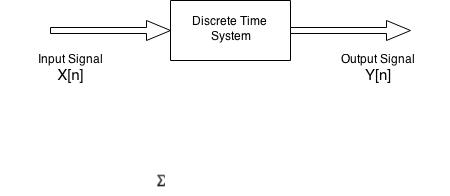
\includegraphics[width=0.7\textwidth]{Block_1.jpg}
\caption{\label{fig:Block_1}Discrete Independent Variable System Representation.}
\end{figure}


\subsection{Examples of a Discrete Time System}

\subsubsection{Example 1}
Consider a Bank Account. 

A certain amount $X[n]$ is deposited at a given time.


$T$ is the interval of interest calculation.


$Y[n]$ is the amount present at the $n$th instant.


The Bank gives an interest half yearly. Thus, a certain amount of interest is calculated after 6 months. The next amount is calculated over the next 6 months.

$\alpha$ is the rate of interest for the first 6 months while $\beta$ will be the rate of interest for the next 6 months. 

Thus if $\alpha$ and $\beta$ are the interest rates over two intervals of 6 months each.

The amount $Y[n]$ at the $n$th instant will be given as:

$$Y[n]=(\alpha.Y[n-1])+(\beta.Y[n-2])+X[n]$$

The amount $Y[n]$ will thus be the interest collected over the previous 2 intervals of 6 months each along with the current amount in the account $X[n]$.

This can be seen as an example of a Discrete System. 

Also, since the output is dependent on it's own past, it is a 'Recursive System'.


\subsubsection{Example 2}
Consider a Population in a region. 

We need to calculated the Tax Paid $Y[n]$ by this population. 

Population (Input) is given by $X[n]$.

The tax is paid over two intervals at the rates $\alpha$ and $\beta$.

The above system can be stated as:

$$Y[n]=(\alpha.X[n])+(\beta.X[n-1])$$

The above system out put or The Tax collected is Independent of it's previous state.

Hence above is a Non-Recursive System.



The Properties of Discrete Independent Variable systems will be studied in the following sessions.


